%2multibyte Version: 5.50.0.2960 CodePage: 65001
% ------------------------------------------------------------
% Macro matematiche ufficiali del progetto MQF
% Coerenti con MQF_Notazione.tex
% ------------------------------------------------------------
% Fallback utile per compilazione esterna se qualche titolo resta scritto come \QTR.
% Scientific WorkPlace usa \QTR internamente; in Beamer \QTR{frametitle}{Titolo}
% deve espandersi in \frametitle{Titolo}.

\documentclass[handout]{beamer}%
\usepackage{mathpazo}
%\usepackage{hyperref}
\usepackage{multimedia}
\usepackage{amsmath}
\usepackage{amsfonts}
\usepackage{amssymb}
\usepackage{graphicx}%
\setcounter{MaxMatrixCols}{30}
%TCIDATA{OutputFilter=latex2.dll}
%TCIDATA{Version=5.50.0.2960}
%TCIDATA{Codepage=65001}
%TCIDATA{CSTFile=beamer.cst}
%TCIDATA{Created=Saturday, May 16, 2026 09:09:59}
%TCIDATA{LastRevised=Saturday, May 16, 2026 11:24:58}
%TCIDATA{<META NAME="GraphicsSave" CONTENT="32">}
%TCIDATA{<META NAME="SaveForMode" CONTENT="2">}
%TCIDATA{BibliographyScheme=Manual}
%TCIDATA{<META NAME="DocumentShell" CONTENT="Other Documents\SW\Slides - Beamer">}
%BeginMSIPreambleData
\graphicspath{{../graphics/}{graphics/}}
\providecommand{\U}[1]{\protect\rule{.1in}{.1in}}
%EndMSIPreambleData
\newenvironment{stepenumerate}{\begin{enumerate}[<+->]}{\end{enumerate}}
\newenvironment{stepitemize}{\begin{itemize}[<+->]}{\end{itemize} }
\newenvironment{stepenumeratewithalert}{\begin{enumerate}[<+-| alert@+>]}{\end{enumerate}}
\newenvironment{stepitemizewithalert}{\begin{itemize}[<+-| alert@+>]}{\end{itemize} }
\usetheme{Madrid}
\providecommand{\R}{\mathbb{R}}
\providecommand{\N}{\mathbb{N}}
\providecommand{\E}{\mathbb{E}}
\providecommand{\Prob}{\mathbb{P}}
\providecommand{\Q}{\mathbb{Q}}
\providecommand{\F}{\mathcal{F}}
\providecommand{\B}{\mathcal{B}}
\providecommand{\G}{\mathcal{G}}
\providecommand{\Var}{\operatorname{Var}}
\providecommand{\Cov}{\operatorname{Cov}}
\providecommand{\VaR}{\operatorname{VaR}}
\providecommand{\CVaR}{\operatorname{CVaR}}
\providecommand{\argmin}{\operatorname*{arg\,min}}
\providecommand{\argmax}{\operatorname*{arg\,max}}
\providecommand{\EVPI}{\operatorname{EVPI}}
\providecommand{\VSS}{\operatorname{VSS}}
\providecommand{\QTR}[2]{\csname #1\endcsname{#2}}
%BeginMSIPreambleData
\ifx\pdfoutput\relax\let\pdfoutput=\undefined\fi
\newcount\msipdfoutput
\ifx\pdfoutput\undefined\else
\ifcase\pdfoutput\else
\msipdfoutput=1
\ifx\paperwidth\undefined\else
\ifdim\paperheight=0pt\relax\else\pdfpageheight\paperheight\fi
\ifdim\paperwidth=0pt\relax\else\pdfpagewidth\paperwidth\fi
\fi\fi\fi
%EndMSIPreambleData


\title{Lezione 1 - Elementi di teoria della probabilit\`{a}}
\subtitle{Metodi Quantitativi per la Finanza}
\author[P. Falbo, C. Pelizzari]{{\LARGE Paolo Falbo, Cristian Pelizzari}}
\institute[]{{\large Dipartimento Economia e Management}}
\date[]{}
\titlegraphic{

\includegraphics[width=3.3cm]{graphics/logo-Unibs-esteso.png}
}

\begin{document}
\maketitle
\section{Apertura}
%****************************************
\subsection{Domanda guida}



%TCIMACRO{\TeXButton{BeginFrame}{\begin{frame}}}%
%BeginExpansion
\begin{frame}%
%EndExpansion

\QTR{frametitle}{Valori attesi condizionati e informazione}

%TCIMACRO{\TeXButton{Transparency}{\setbeamercovered{transparent=20}}}%
%BeginExpansion
\setbeamercovered{transparent=20}%
%EndExpansion

\begin{center}
{\Large Come cambia una media quando cambia l'informazione?}
\end{center}

\medskip

In finanza una valutazione non dipende solo dal payoff futuro, ma anche
dall'informazione disponibile al momento della decisione.

\medskip

\begin{stepitemize}
\item senza informazione aggiuntiva si valuta una media non condizionata;

\item osservando un evento rilevante, la distribuzione dei possibili esiti cambia;

\item osservando una partizione informativa, la valutazione diventa diversa
nei diversi stati osservabili;

\item il valore atteso condizionato formalizza questa revisione:
\[
\E[H\mid\G].
\]
\end{stepitemize}

\medskip

%TCIMACRO{\TeXButton{Transition: Box Out}{\transboxout}}%
%BeginExpansion
\transboxout%
%EndExpansion
%TCIMACRO{\TeXButton{EndFrame}{\end{frame}}}%
%BeginExpansion
\end{frame}%
%EndExpansion

\subsection{Obiettivi della lezione}

%****************************************
%TCIMACRO{\TeXButton{BeginFrame}{\begin{frame}}}%
%BeginExpansion
\begin{frame}%
%EndExpansion

\QTR{frametitle}{Obiettivi della lezione}

%TCIMACRO{\TeXButton{Transparency}{\setbeamercovered{transparent=20}}}%
%BeginExpansion
\setbeamercovered{transparent=20}%
%EndExpansion

Al termine della lezione lo studente deve saper interpretare il valore
atteso condizionato come valutazione coerente con l'informazione disponibile.

\medskip

\begin{stepitemize}
\item richiamare probabilit\`{a} condizionata e distribuzione condizionata;

\item calcolare un valore atteso condizionato rispetto a un evento:
\[
\E[H\mid A];
\]

\item passare da eventi e partizioni a sigma-algebre informative:
\[
\G\subseteq\F;
\]

\item interpretare il valore atteso condizionato come variabile casuale:
\[
\E[H\mid\G];
\]

\item usare le principali regole operative e applicarle a payoff e perdite finanziarie.
\end{stepitemize}

%TCIMACRO{\TeXButton{Transition: Box Out}{\transboxout}}%
%BeginExpansion
\transboxout%
%EndExpansion
%TCIMACRO{\TeXButton{EndFrame}{\end{frame}}}%
%BeginExpansion
\end{frame}%
%EndExpansion
%***********************************

\subsection{Obiettivi della lezione}
%TCIMACRO{\TeXButton{BeginFrame}{\begin{frame}}}%
%BeginExpansion
\begin{frame}%
%EndExpansion

\QTR{frametitle}{Obiettivi della lezione}

%TCIMACRO{\TeXButton{Transparency}{\setbeamercovered{transparent=20}}}%
%BeginExpansion
\setbeamercovered{transparent=20}%
%EndExpansion

Al termine della lezione dovremo saper interpretare il valore atteso
condizionato come valutazione coerente con una data informazione.

\medskip

\begin{stepenumerate}
\item [1.] Richiamare probabilit\`{a} condizionata e distribuzione condizionata
rispetto a un evento osservato.

\item [2.] Definire il valore atteso condizionato rispetto a un evento:
\[
\E[X\mid A].
\]

\item [3.] Passare da eventi singoli a partizioni informative e alla
sigma-algebra generata:
\[
\G=\sigma(B_1,\ldots,B_n).
\]

\item [4.] Interpretare $\E[X\mid\G]$ come variabile casuale osservabile
rispetto all'informazione disponibile.

\item [5.] Usare le principali regole operative e applicarle a payoff,
perdite e scenari di mercato.
\end{stepenumerate}

%TCIMACRO{\TeXButton{Transition: Box Out}{\transboxout}}%
%BeginExpansion
\transboxout%
%EndExpansion
%TCIMACRO{\TeXButton{EndFrame}{\end{frame}}}%
%BeginExpansion
\end{frame}%
%EndExpansion
%*********************************************

%TCIMACRO{\TeXButton{BeginFrame}{\begin{frame}}}%
%BeginExpansion
\begin{frame}%
%EndExpansion

\QTR{frametitle}{Motivazione finanziaria}

%TCIMACRO{\TeXButton{Transparency}{\setbeamercovered{transparent=20}}}%
%BeginExpansion
\setbeamercovered{transparent=20}%
%EndExpansion

Molte grandezze finanziarie sono valutate prima che l'incertezza sia
risolta.

\medskip

\begin{stepitemize}
\item Un \textbf{payoff} futuro $H$ dipende dallo stato di mercato che si
realizzer\`{a}.

\item Una \textbf{perdita} futura $L$ dipende da prezzi, tassi, default e
fattori di rischio non ancora osservati.

\item La valutazione iniziale usa l'informazione disponibile oggi:
\[
\E[H], \qquad \E[L].
\]

\item Se arriva nuova informazione, la valutazione deve essere aggiornata:
\[
\E[H\mid \G], \qquad \E[L\mid \G].
\]
\end{stepitemize}

\medskip

\begin{center}
{\small Condizionare significa valutare una grandezza incerta alla luce
dell'informazione osservabile.}
\end{center}

%TCIMACRO{\TeXButton{Transition: Box Out}{\transboxout}}%
%BeginExpansion
\transboxout%
%EndExpansion
%TCIMACRO{\TeXButton{EndFrame}{\end{frame}}}%
%BeginExpansion
\end{frame}%
%EndExpansion
%*********************************************

\subsection{L'informazione cambia i pesi}
%TCIMACRO{\TeXButton{BeginFrame}{\begin{frame}}}%
%BeginExpansion
\begin{frame}%
%EndExpansion

\QTR{frametitle}{L'informazione cambia i pesi}

%TCIMACRO{\TeXButton{Transparency}{\setbeamercovered{transparent=20}}}%
%BeginExpansion
\setbeamercovered{transparent=20}%
%EndExpansion

Condizionare rispetto ad un evento \textbf{non cambia} il payoff di $H$: cambia l'insieme degli scenari ritenuti compatibili con l'informazione osservata.

\medskip

\begin{stepitemize}
\item Prima dell'informazione, ogni scenario $\omega\in\Omega$ contribuisce
secondo la probabilit\`{a} iniziale $\Prob$.

\item Dopo l'osservazione di un evento $A$, restano rilevanti solo gli
scenari compatibili:
\[
\omega\in A.
\]

\item La media viene ricalcolata usando le \textbf{probabilit\`{a}
condizionate}:
\[
\Prob(H \in,\cdot\,\mid A).
\]

\item Quindi non si modifica la funzione payoff $H$, ma la
\textbf{distribuzione} rispetto alla quale $H$ viene valutato.
\end{stepitemize}


%TCIMACRO{\TeXButton{Transition: Box Out}{\transboxout}}%
%BeginExpansion
\transboxout%
%EndExpansion
%TCIMACRO{\TeXButton{EndFrame}{\end{frame}}}%
%BeginExpansion
\end{frame}%
%EndExpansion
%*********************************************

\subsection{Valore atteso condizionato rispetto a un evento}
%TCIMACRO{\TeXButton{BeginFrame}{\begin{frame}}}%
%BeginExpansion
\begin{frame}%
%EndExpansion

\QTR{frametitle}{Valore atteso condizionato rispetto a un evento}

%TCIMACRO{\TeXButton{Transparency}{\setbeamercovered{transparent=20}}}%
%BeginExpansion
\setbeamercovered{transparent=20}%
%EndExpansion

Sia $H$ una variabile casuale discreta e sia $A\in\F$ un evento con
$\Prob(A)>0$.

\medskip

\begin{stepitemize}
\item Il valore atteso condizionato rispetto ad $A$ \`{e}:
\[
\E[H\mid A]=\sum_h h\,\Prob(H=h\mid A).
\]

\item I pesi della media sono le \textbf{probabilit\`{a} condizionate}:
\[
\Prob(H=h\mid A)
=
\frac{\Prob(\{H=h\}\cap A)}{\Prob(A)}.
\]

\item L'evento $A$ seleziona l'informazione osservata; la media considera
solo gli esiti di $H$ coerenti con tale informazione.

\item $\E[H\mid A]$ \`{e} un numero: rappresenta la valutazione media di
$H$ dopo aver osservato $A$.
\end{stepitemize}

%TCIMACRO{\TeXButton{Transition: Box Out}{\transboxout}}%
%BeginExpansion
\transboxout%
%EndExpansion
%TCIMACRO{\TeXButton{EndFrame}{\end{frame}}}%
%BeginExpansion
\end{frame}%
%EndExpansion
%*********************************************

\subsection{Formula con indicatrice}
%TCIMACRO{\TeXButton{BeginFrame}{\begin{frame}}}%
%BeginExpansion
\begin{frame}%
%EndExpansion

\QTR{frametitle}{Formula con indicatrice}

%TCIMACRO{\TeXButton{Transparency}{\setbeamercovered{transparent=20}}}%
%BeginExpansion
\setbeamercovered{transparent=20}%
%EndExpansion

Sia $A\in\F$ un evento con probabilit\`{a} positiva:
\[
\Prob(A)>0.
\]

\medskip

Il valore atteso condizionato di $X$ dato $A$ pu\`{o} essere scritto come:
\[
\E[X\mid A]
=
\frac{\E[X\mathbf{1}_{A}]}{\Prob(A)}.
\]

\medskip

\begin{stepitemize}
\item $\mathbf{1}_{A}$ seleziona gli scenari in cui l'evento $A$ si verifica.

\item $\E[X\mathbf{1}_{A}]$ somma il contributo di $X$ solo sugli scenari
compatibili con $A$.

\item La divisione per $\Prob(A)$ normalizza la media rispetto alla
probabilit\`{a} dell'evento condizionante.
\end{stepitemize}

\medskip

\begin{center}
{\small La formula mostra che condizionare equivale a restringere e
rinormalizzare la valutazione.}
\end{center}

%TCIMACRO{\TeXButton{Transition: Box Out}{\transboxout}}%
%BeginExpansion
\transboxout%
%EndExpansion
%TCIMACRO{\TeXButton{EndFrame}{\end{frame}}}%
%BeginExpansion
\end{frame}%
%EndExpansion
%*********************************************

\subsection{Caso continuo}
%TCIMACRO{\TeXButton{BeginFrame}{\begin{frame}}}%
%BeginExpansion
\begin{frame}%
%EndExpansion

\QTR{frametitle}{Caso continuo}

%TCIMACRO{\TeXButton{Transparency}{\setbeamercovered{transparent=20}}}%
%BeginExpansion
\setbeamercovered{transparent=20}%
%EndExpansion

Nel caso continuo il condizionamento modifica la \textbf{densit\`{a}}
rispetto alla quale si calcola la media.

\medskip

Se $X$ ha densit\`{a} condizionata $f_{X\mid A}$ dato l'evento $A$, allora:
\[
\E[X\mid A]
=
\int_{\R} x f_{X\mid A}(x)\,dx.
\]

\medskip

\begin{stepitemize}
\item La funzione $f_{X\mid A}$ descrive la distribuzione di $X$ dopo
l'osservazione di $A$.

\item L'integrale \`{e} la stessa operazione di media, ma calcolata con i
\textbf{pesi condizionati}.

\item La grandezza $X$ non viene modificata: cambia la distribuzione
rilevante per la sua valutazione.
\end{stepitemize}

%TCIMACRO{\TeXButton{Transition: Box Out}{\transboxout}}%
%BeginExpansion
\transboxout%
%EndExpansion
%TCIMACRO{\TeXButton{EndFrame}{\end{frame}}}%
%BeginExpansion
\end{frame}%
%EndExpansion

%*************************************

\subsection{Partizioni informative}
%TCIMACRO{\TeXButton{BeginFrame}{\begin{frame}}}%
%BeginExpansion
\begin{frame}%
%EndExpansion

\QTR{frametitle}{Partizioni informative}

%TCIMACRO{\TeXButton{Transparency}{\setbeamercovered{transparent=20}}}%
%BeginExpansion
\setbeamercovered{transparent=20}%
%EndExpansion

Una \textbf{partizione informativa} descrive gli stati che diventano
distinguibili dopo l'osservazione di un segnale.

\medskip

Sia
\[
\Omega = B_1\cup\cdots\cup B_n,
\qquad
B_i\cap B_j=\varnothing \quad \text{se } i\neq j.
\]

\begin{stepitemize}
\item Prima dell'osservazione non sappiamo quale blocco $B_i$ si
realizzer\`{a}.

\item Dopo l'osservazione sappiamo che lo scenario vero appartiene a uno
specifico blocco $B_i$.

\item Per ciascun blocco possiamo calcolare una \textbf{media locale}:
\[
\E[X\mid B_i].
\]

\item La partizione trasforma una sola valutazione globale in una famiglia
di valutazioni condizionate.
\end{stepitemize}

%TCIMACRO{\TeXButton{Transition: Box Out}{\transboxout}}%
%BeginExpansion
\transboxout%
%EndExpansion
%TCIMACRO{\TeXButton{EndFrame}{\end{frame}}}%
%BeginExpansion
\end{frame}%
%EndExpansion
%*********************************************

\subsection{Valore atteso totale}
%TCIMACRO{\TeXButton{BeginFrame}{\begin{frame}}}%
%BeginExpansion
\begin{frame}%
%EndExpansion

\QTR{frametitle}{Valore atteso totale}

%TCIMACRO{\TeXButton{Transparency}{\setbeamercovered{transparent=20}}}%
%BeginExpansion
\setbeamercovered{transparent=20}%
%EndExpansion

La media non condizionata si ottiene ricomponendo le medie locali sui
blocchi della partizione.

\medskip

Se $\{B_1,\ldots,B_n\}$ \`{e} una partizione di $\Omega$ e
$\Prob(B_i)>0$, allora:
\[
\E[X]
=
\sum_{i=1}^{n}\E[X\mid B_i]\Prob(B_i).
\]

\medskip

\begin{stepitemize}
\item $\E[X\mid B_i]$ \`{e} la valutazione di $X$ quando l'informazione
osservata identifica il blocco $B_i$.

\item $\Prob(B_i)$ \`{e} il peso ex ante attribuito a quel possibile stato
informativo.

\item La media globale \`{e} quindi una \textbf{media ponderata} delle
valutazioni condizionate.
\end{stepitemize}

\medskip

\begin{center}
{\small Il valore atteso totale collega la valutazione prima
dell'informazione alle valutazioni dopo l'informazione.}
\end{center}

%TCIMACRO{\TeXButton{Transition: Box Out}{\transboxout}}%
%BeginExpansion
\transboxout%
%EndExpansion
%TCIMACRO{\TeXButton{EndFrame}{\end{frame}}}%
%BeginExpansion
\end{frame}%
%EndExpansion
%*********************************************

\subsection{Figura 3.1: partizione di Omega}
%TCIMACRO{\TeXButton{BeginFrame}{\begin{frame}}}%
%BeginExpansion
\begin{frame}%
%EndExpansion

\QTR{frametitle}{Figura 3.1: partizione di $\Omega$}

%TCIMACRO{\TeXButton{Transparency}{\setbeamercovered{transparent=20}}}%
%BeginExpansion
\setbeamercovered{transparent=20}%
%EndExpansion

\begin{center}
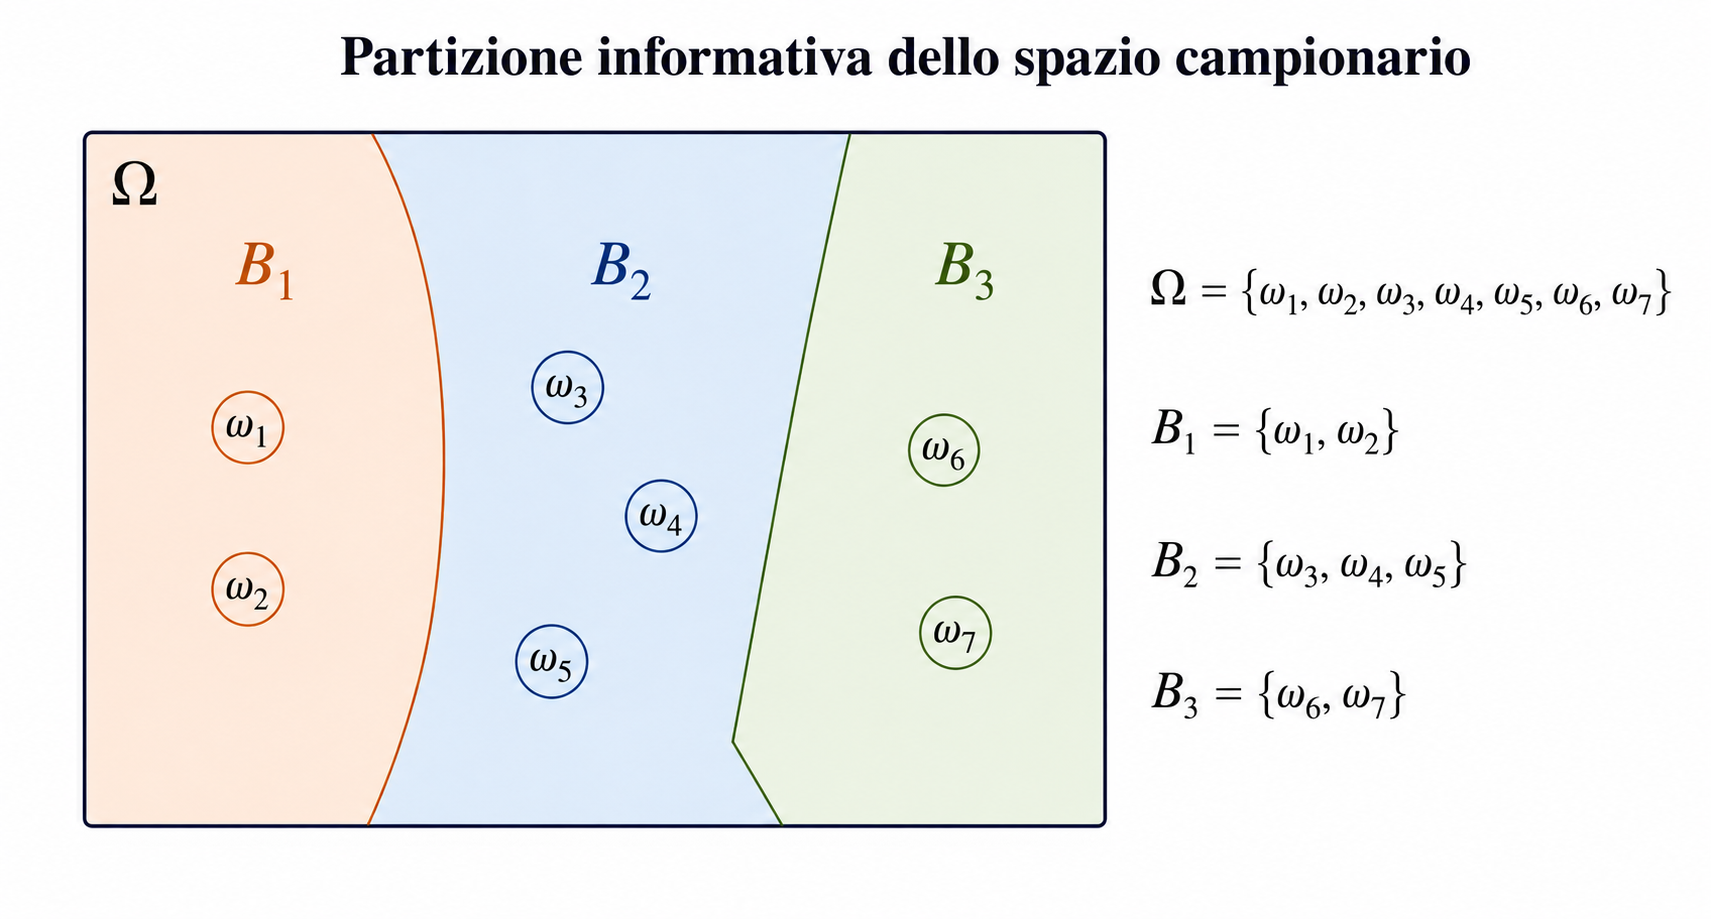
\includegraphics[width=0.72\textwidth]{../graphics/Figura_3_1.png}
\end{center}

\begin{stepitemize}
\item Gli eventi elementari rappresentano i singoli scenari $\omega\in\Omega$.

\item Gli eventi $B_1,\ldots,B_n$ raccolgono scenari elementari non distinguibili
dalla stessa \textbf{informazione osservata}.

\item Osservare la partizione significa sapere quale evento $B_i$ si \`{e}
realizzato, senza necessariamente identificare il singolo scenario
elementare $\omega$.
\end{stepitemize}

%TCIMACRO{\TeXButton{Transition: Box Out}{\transboxout}}%
%BeginExpansion
\transboxout%
%EndExpansion
%TCIMACRO{\TeXButton{EndFrame}{\end{frame}}}%
%BeginExpansion
\end{frame}%
%EndExpansion
%*********************************************






%***********************************
\end{document}